\documentclass[10pt,a4paper,english]{article}

\usepackage[utf8]{inputenc}
\usepackage{graphicx}
\usepackage{amsmath}
\usepackage{float}
\usepackage{parskip}

\title{System overview}
\author{\begin{large}{Robotics Safety}\end{large}\\\\
Olle Fridolfsson (ollfr940) \\  Niklas Hansson (nikha310) \\ Patrik Hillgren (pathi747) \\ Benjamin Ingberg (benin542)\\ Pär Lundgren (parlu048) \\ Mattias Nilsson (matni796)}

\setcounter{secnumdepth}{1}
\setcounter{tocdepth}{3}

\begin{document}
\maketitle
\centerline {Responsible editor: Olle Fridolfsson}
\clearpage
\tableofcontents
\clearpage
\section{Basic overview}

The system will consist of four major parts which will work together to allow an industrial robot to safely work in an environment where people might enter and exit its workspace.

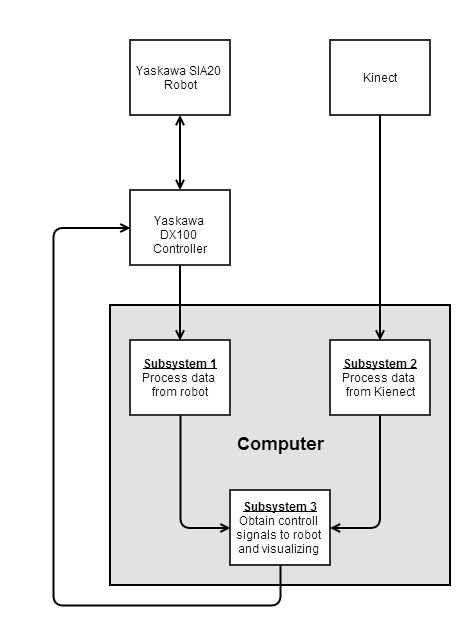
\includegraphics[width=\columnwidth]{robot_safety.jpg}

\subsection{Kinect camera system}

External information will come from a Kinect camera system which contains several sensors.\cite{kinectref}

\begin{itemize}
\item Three channel RGB-camera
\item An infrared (IR) emitter and IR-camera which together forms a stereo depth image in the IR-spectrum.
\item A multi-array microphone which is capable of determining from which direction the sound originates. Will most likely not be used in the project.
\item A 3-axis accelerometer capable of determining the orientation of the Kinect in relation to the gravitational pull.
\end{itemize}

\subsection{Yaskawa SIA20 robot}

The Yaskawa SIA20 is a seven-axis robot for industrial manufacturing which is connected to the computer system via a controller.\cite{sia20}

\subsection{Yaskawa DX100 controller}

The Yaskawa DX100 controller is based on Windows CE, it can control up to 72 axises at the same time. It has a touch screen which allows the user to perform manual based programming. By teaching the robot a set of moves it can be programmed to perform a continuous movement pattern.

\section{Subsystem overview}

The computational system will consist of several subsystems which handle different parts of the algorithms.

\subsection{Subsystem 1 - Robot data processing}

The robot data subsystem will abstract the robots positions to a 3d-model according to the internal state of the robot from the controller.

\subsubsection{Transformation of robot data}

The transmitted data from the controller describing the state of the different robot axes must be transformed into a known coordinate system.

Most likely this will be done using the Relative Job solution initialized with a base coordinate system (i.e. at the ground, centered at the robot). In a relative job a postion will be given in a 3D world coordinate system. In a standard job the orientation of the robot is given by the axises revolutions.  

\subsubsection{3d-model}

The transformed robot data will be used to create a 3d-model of the robot. From this data we will subsequently be able to construct the safety regions.

\subsection{Subsystem 2 - Camera data processing}

From the camera system there will be a depth image and possibly a color image that has to be calibrated and processed to build 3d-models which separate background from foreground.

\subsubsection{Calibration}

The camera system has to be calibrated, this will be done by using chessboard patterns. The calibration will take into consideration radial and tangential distortions using OpenCV's distortion models.

By taking several pictures using a chessboard pattern in different angles the intrinsic camera parameters can be estimated. Since the intrinsic parameters should be constant, this will only have to be done before installation. Afterwards the camera extrinsic parameters can be extrapolated by solving the perspective n-point (PnP) problem for a pattern which has a fix relation to the robot's coordinate system.

By covering the kinect's IR-projector, either through software or mechanically, and looking directly at the IR-image the same methodology can be used to calibrate the depth camera.
These standard algorithms are already implemented in Open CV.\cite{opencv-calibration}

\subsubsection{Background modelling and segmentation}

Regions of the images corresponding to background and foreground will have to be separated. For this a statistical background model will be used.

There are several available background models implemented in Open CV with differing performance and suitability. Based on initial trials, one of these will be chosen.

\subsection{Subsystem 3 - Merging subsystem}

The merging subsystem takes information from the two previous subsystems and performs the necessary calculations to determine distance between the robot position (as determined from the internal robot state) and the detected objects (as determined from the background modelling and the depth camera).

\subsubsection{Merging of 3d-data}

There will be data available from the two previous subsystems regarding the robot and its environment. 

This data will be combined to determine if there is any movement in the robot safety regions. The robot itself and any objects moving in predetermined safety areas will be excluded from this.

\subsubsection{Visualization}

Visualization will be crucial to understand this system, since the depth camera gives us a point-cloud and the image camera gives us a texture for the point cloud. A 3d-visualization will be implemented with OpenGL. Using information from the background model it will be possible to visualize regions that are occluded.

\subsubsection{Robot control signals}

If any objects are detected in the safety areas, appropriate control signals will be sent to the robot forcing it to slow down or come to a complete halt.

\clearpage

\begin{thebibliography}{9}

\bibitem{kinectref}
Microsofts specification of Kinect sensors

http://msdn.microsoft.com/en-us/library/jj131033.aspx

\bibitem{sia20}
Yaskawa datasheet for the SIA20 robot

http://www.motoman.com/datasheets/SIA20D.pdf

\bibitem{opencv-calibration}
OpenCV documentation on calibration

http://docs.opencv.org/modules/calib3d/doc/camera\_calibration\_and\_3d\_reconstruction.html


\end{thebibliography}

\end{document}